
\frontmatter
% \frenchspacing
\onehalfspacing
% \RaggedRight


%  Cabeçalho, rodapé, seção, capítulo e paginação

\makeatletter
\apptocmd{\@part}{\parttitle{#2}}{}{}
\def\parttitle#1{\gdef\theparttitle{#1}}
\def\theparttitle{} % initialization
\makeatother

\pagestyle{scrheadings}
\clearscrheadfoot
\automark[section]{chapter}
\ohead*{\pagemark}
\ofoot{\Ifthispageodd{\leftmark}{\rightmark}}
% \ifoot[\theparttitle]{\theparttitle}




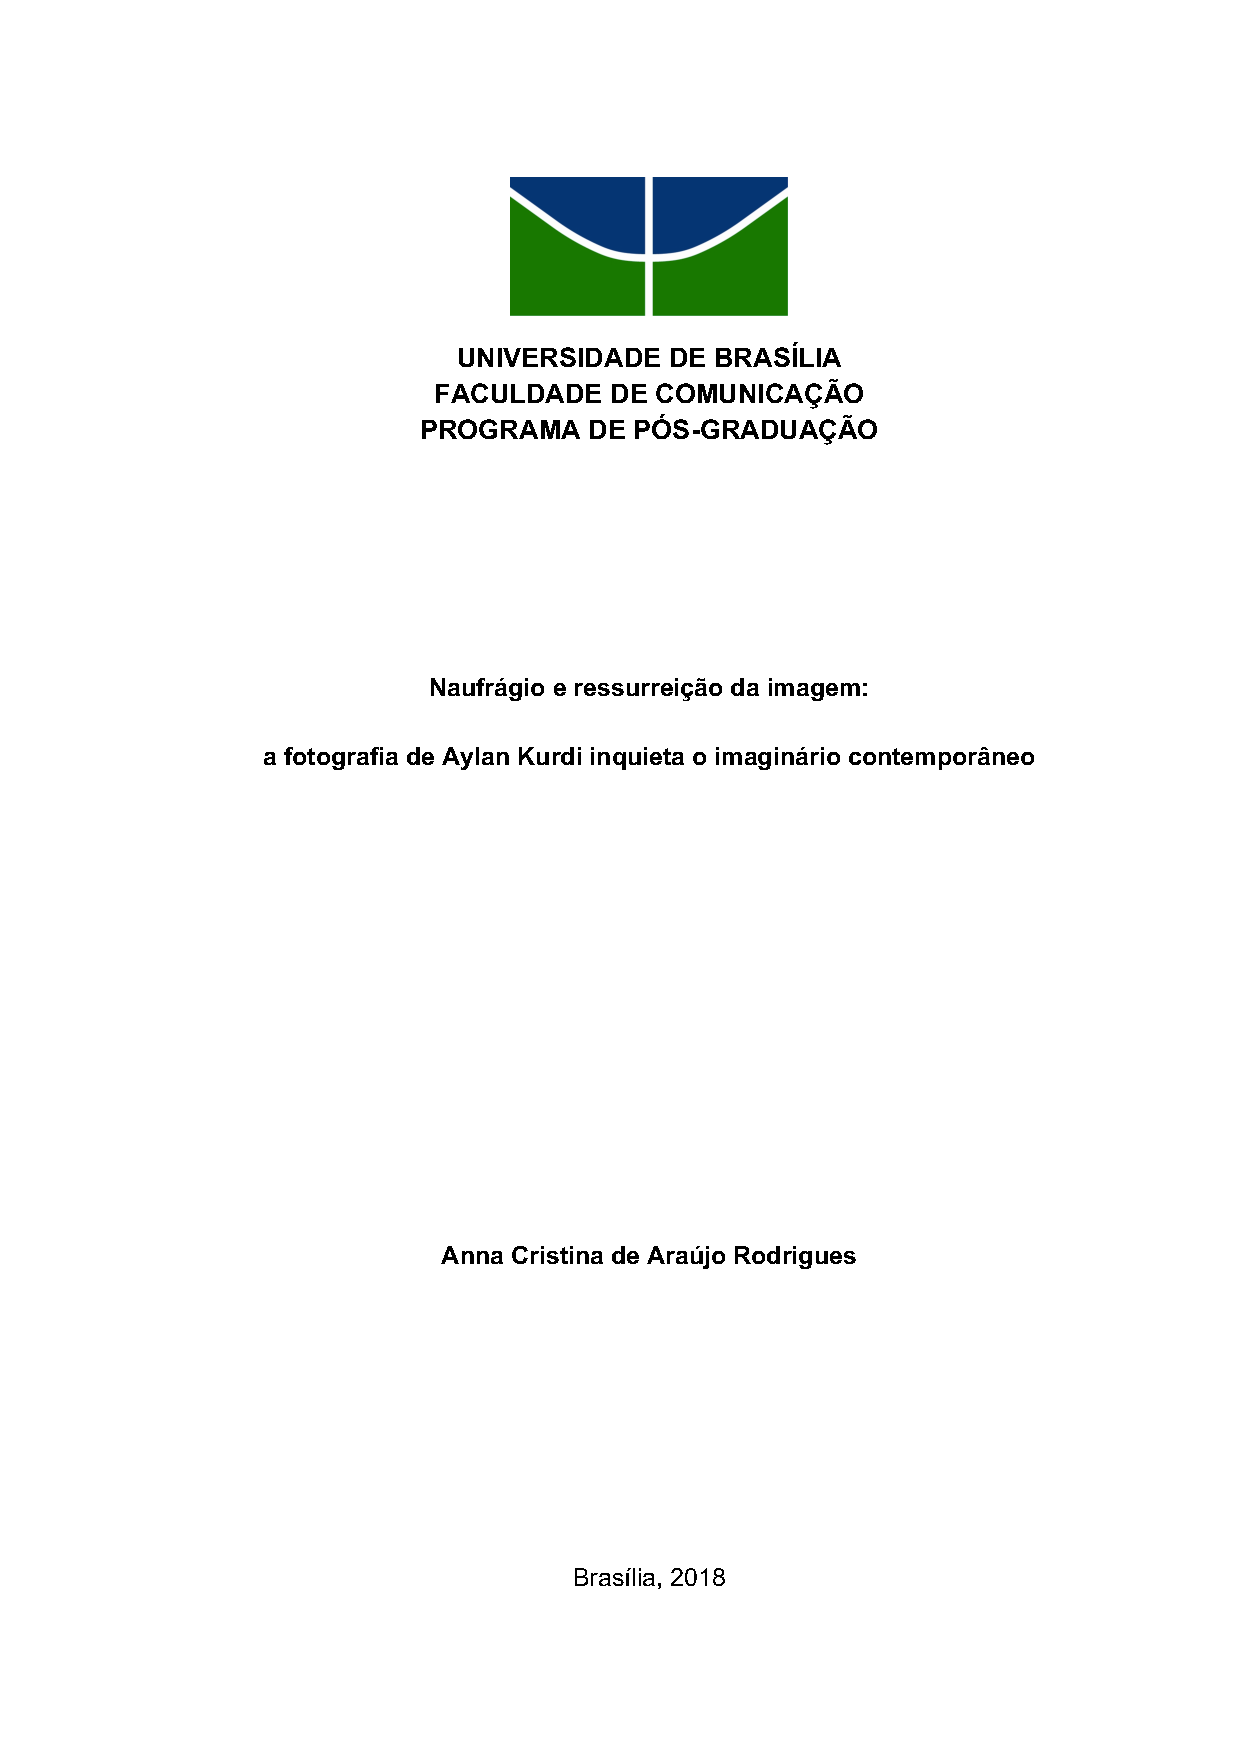
\includepdf{imgs/capa.pdf}
\pagebreak
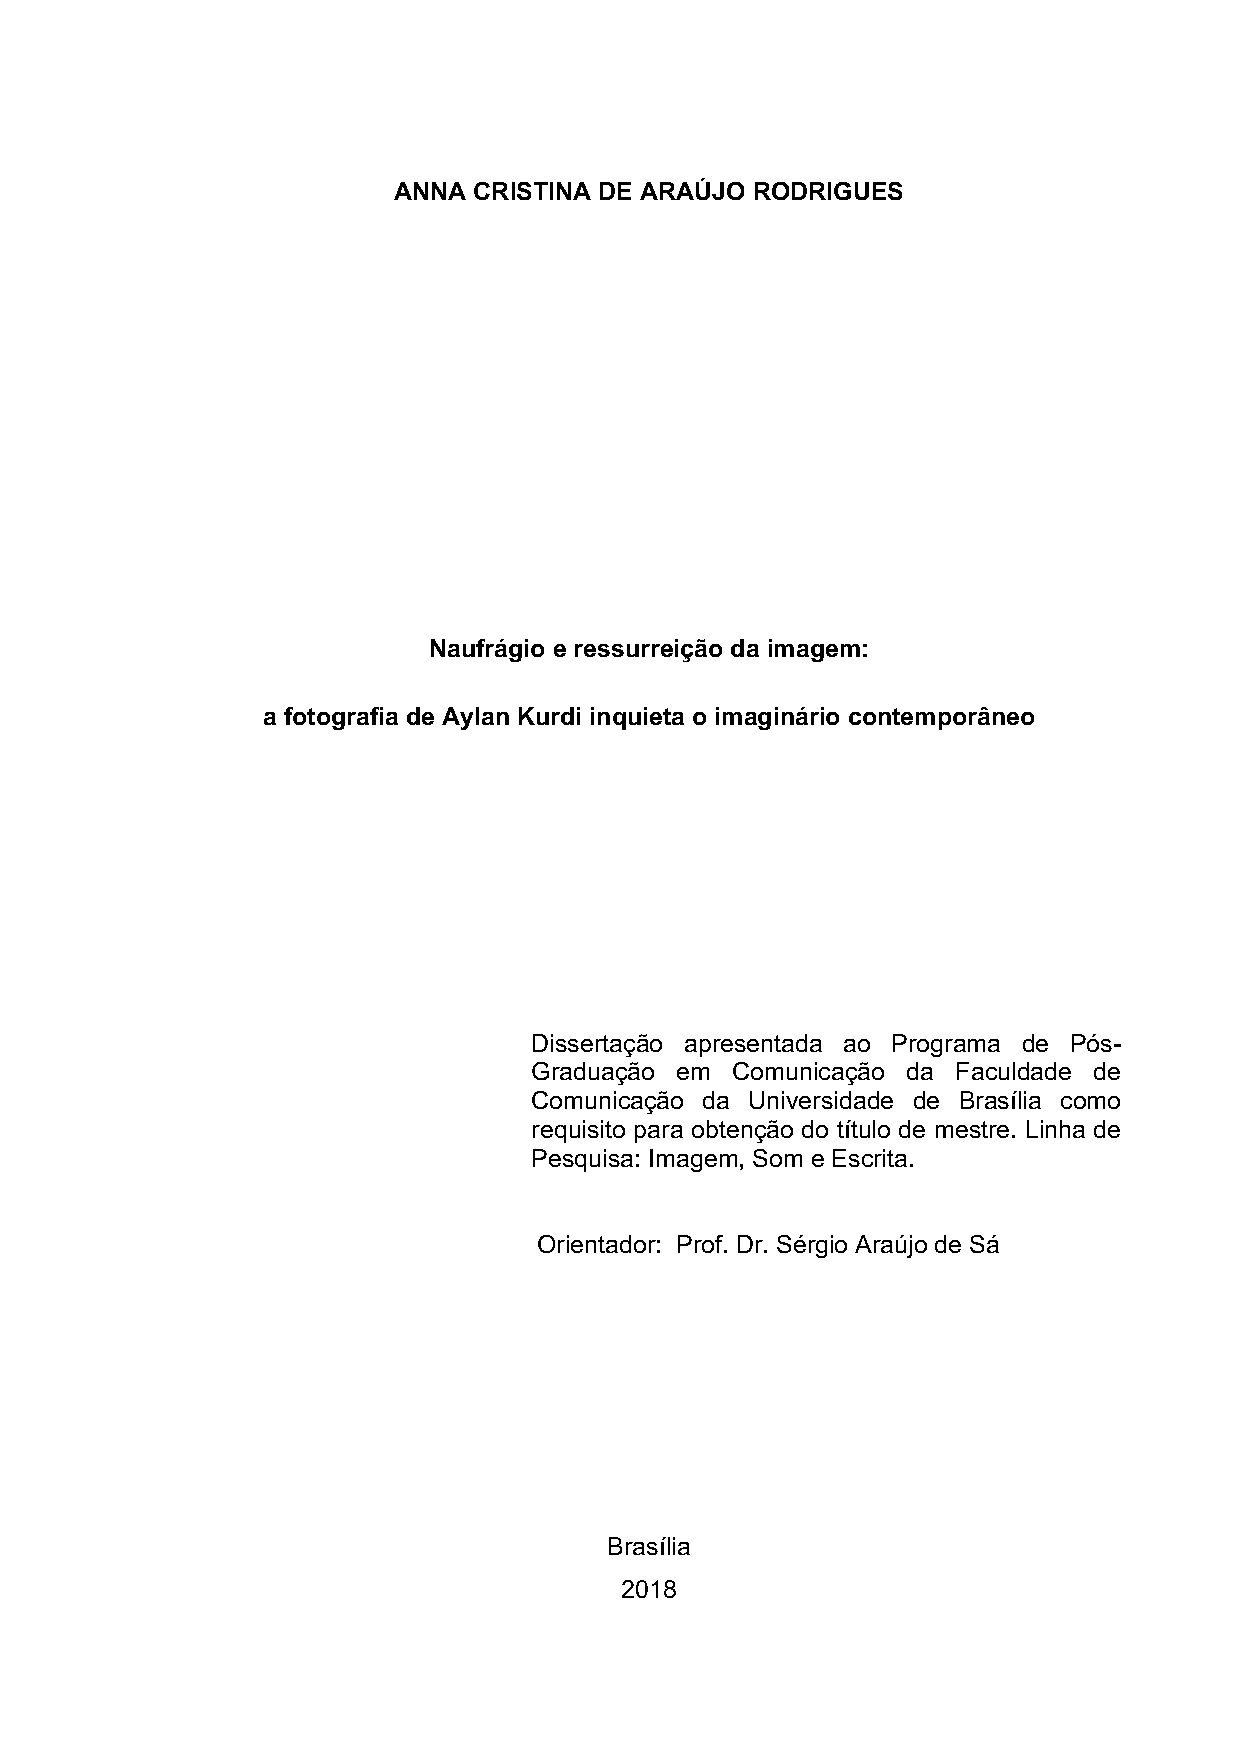
\includepdf{imgs/folha_de_rosto.pdf}
\pagebreak
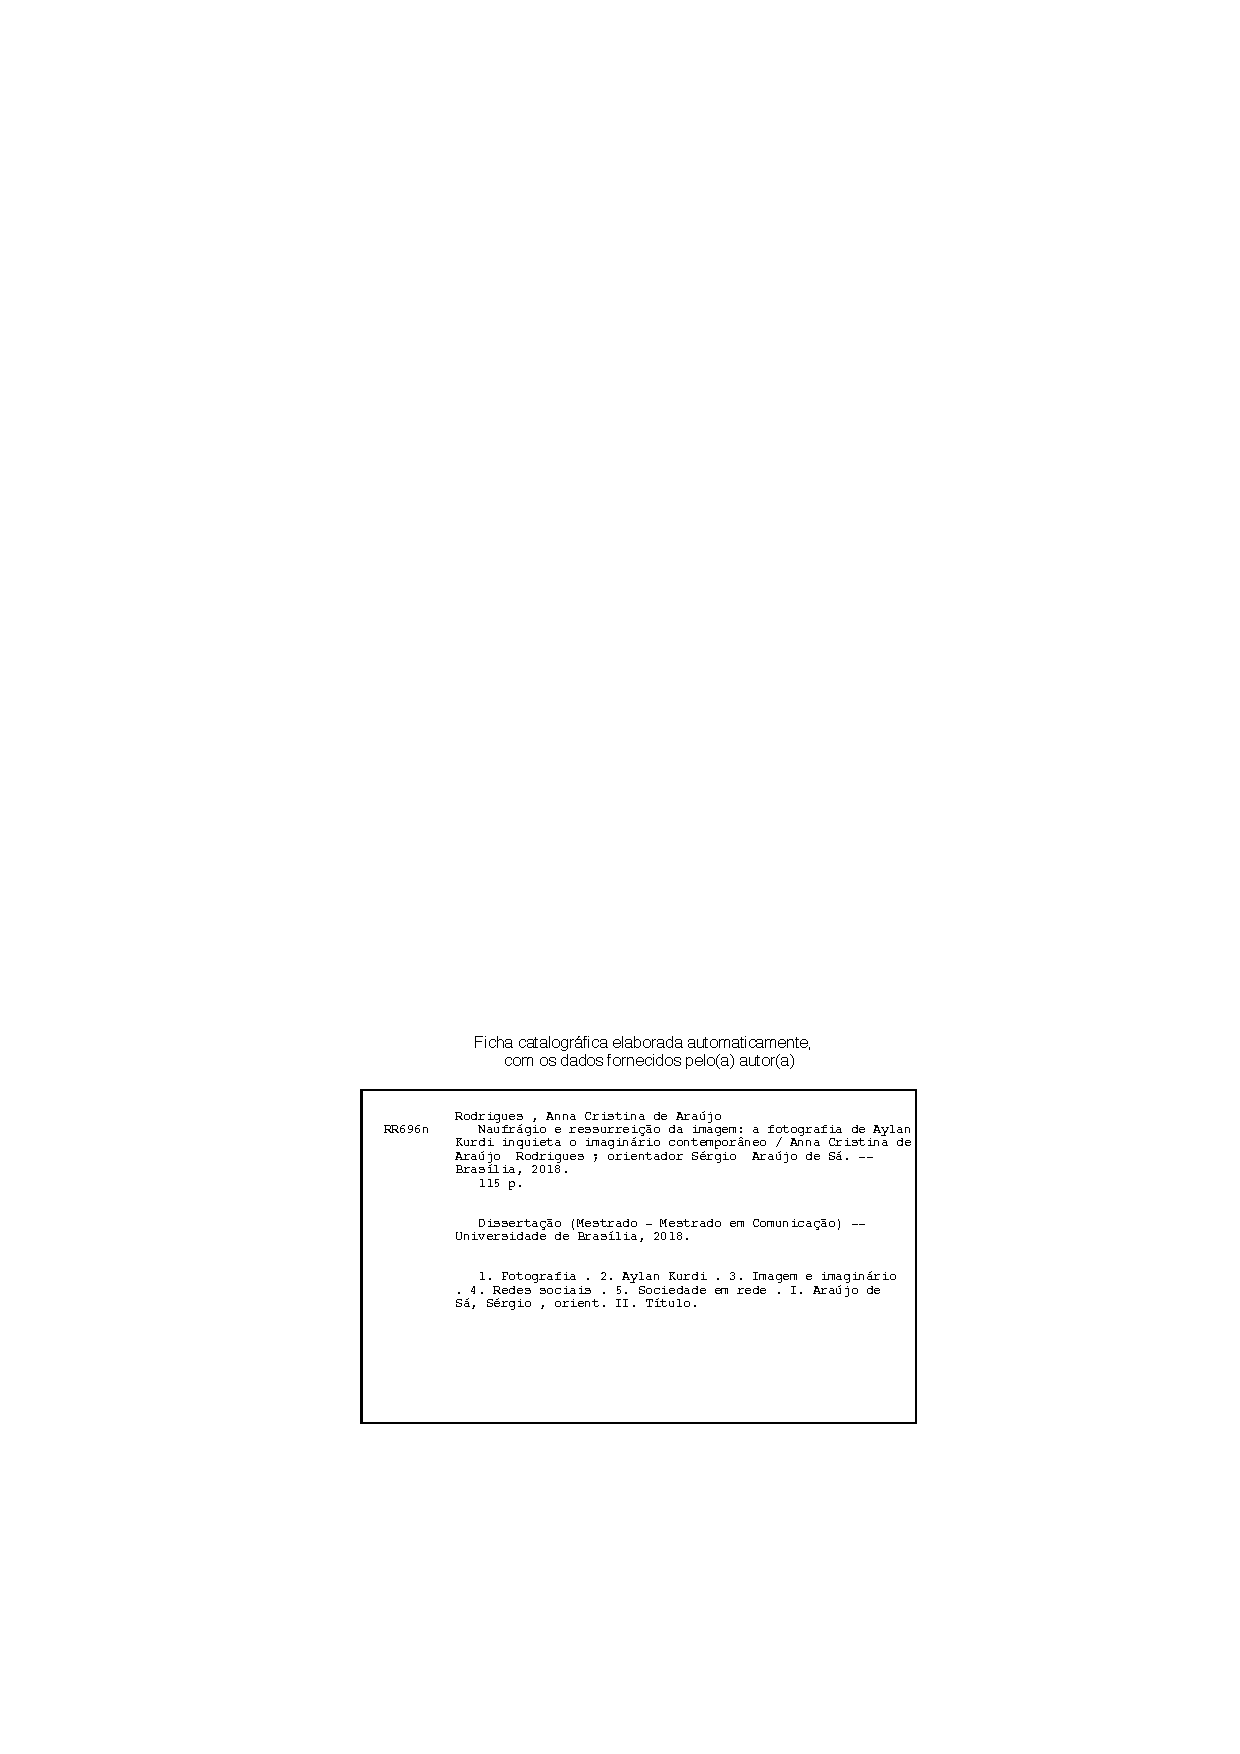
\includepdf{imgs/ficha_catalografica.pdf}
% \author{$author$}
% \title{$title$}
% \def\degreetitle{$degreetype$}
% \degrees{$degrees$}
% \def\affiliation{$affiliation$}

% % Add subject and keywords below
% \hypersetup{
%      %pdfsubject={The Subject},
%      %pdfkeywords={Some Keywords},
%      pdfauthor={$author$},
%      pdftitle={$title$},
%      pdfproducer={Quarto with LaTeX}
% }



% \titulo{Modelo Canônico de\\ Trabalho Acadêmico com \abnTeX}
% \autor{Equipe \abnTeX}
% \local{Brasil}
% \data{2014, v-1.9.2}
% \orientador{Lauro César Araujo}
% \coorientador{Equipe \abnTeX}
% \instituicao{%
%   Universidade do Brasil -- UBr
%   \par
%   Faculdade de Arquitetura da Informação
%   \par
%   Programa de Pós-Graduação}
% \tipotrabalho{Tese (Doutorado)}
% % O preambulo deve conter o tipo do trabalho, o objetivo, 
% % o nome da instituição e a área de concentração 
% \preambulo{Modelo canônico de trabalho monográfico acadêmico em conformidade com
% as normas ABNT apresentado à comunidade de usuários \LaTeX.}